\section{Analysis: RMSE vs Spike Rate for Constant Driving Force}




We analyse the network described by equations (\ref{eq:rotated_voltage_dynamics}) and (\ref{eq:rho_dot}) for the case of a constant (in time) driving force $c(\xi) = k$. First we derive explicit expressions for the network estimate, then we compute the resulting RMSE for various driving strengths $k$.\\
\begin{enumerate}
\item Let 
\begin{align*}
A &= -\begin{bmatrix}  
1 & 0 \\
0 & 1
\end{bmatrix} = \Lambda,\notag \\
\notag \\
B &= \begin{bmatrix}  
1 & 0 \\
0 & 1
\end{bmatrix} = I, \notag \\
\notag \\
D
&=
\mathcal{U} 
\begin{bmatrix}
S & 0
\end{bmatrix}
V^T
=
\mathcal{U} 
\begin{bmatrix}
I_d & 0
\end{bmatrix}
I_N \notag,
\\
\\
c(\xi) &= k \in \mathbf{R}^d, \text{expressed in the $\mathcal{U}-V$ basis},\\
\notag \\
d\xi &= 10^{-4},\notag \\
\notag \\
N &= 4,\notag \\
\notag \\
x(0) &= \begin{bmatrix} \frac{1}{2} & 0 \end{bmatrix}.\notag 
\end{align*}

The system simplifies to one neuron by noting the following: The voltage of the $2d$ non trivial neurons is 
$$
v = S \epsilon.
$$
Voltage $j$ spikes i.f.f. $v_j = \frac{||S_j||^2}{2}$. Let $1$ index the neuron whose encoding direction $S_j$ is closest in angle to $k$, i.e
\begin{align*}
S_1^T e &\geq S_j^T e \hspace{2mm} \forall \, j
\\
\\
\implies v_1 &\geq v_k \hspace{2mm} \forall \, j.
\end{align*}
It follows from equation (\ref{eq:rotated_voltage_dynamics}) that $v_1$ will reach its threshold first. Neuron $1$ spikes and its voltage is reset, and sequence repeats.
Let us integrate until the first spike, avoiding the discontinuity from $\tilde{o}$. The nontrivial dynamics simplify to 
\begin{align}
\label{eq:simple_voltage_dynamics_constant_driving}
\dot{v_1}(\xi) &= \Lambda_1 v_1(\xi) + (\Lambda_1 + 1)||S_1||^2 \rho_1(\xi) + S_1^T k, \notag
\\
\\ \notag
\dot{\rho_1}(\xi) &= -\rho_1(\xi).
\end{align}
With initial conditions $v_1(0)=v_1^0$ and $\rho_1(0)=\rho_1^0,$ the system of equations has the general solution

\begin{align}
\rho_1(\xi) &= \rho_1^0 e^{-\xi}, \notag
\\
\\ \notag
v_1(\xi) 
&=
e^{\Lambda_1 \xi}  \left(\frac{S_1^T k}{\Lambda_1}+ ||S_1||^2 \rho_1^0 + v_1^0\right) - e^{-\xi} \,||S_1||^2 \, \rho_1^0 - \frac{S_1^T k}{\Lambda_1}.
\end{align}

Between spikes, neuron $1$'s voltage is independent from other neurons $j$. The voltage $v_1$ only depends on its own history and feedback from its own spike train, $\rho_1$. Replace index $1$ we see this is true for all neurons so that all neurons are \textit{self-coupled}, hence the name. 

A spike occurs when $v(\xi_{spike}) = \frac{||S_1||^2}{2}$, or

\begin{align*}
\frac{||S_1||^2}{2} 
&=
e^{\Lambda_1 \xi_{spike}}  \left(\frac{S_1^T k}{\Lambda_1}+ ||S_1||^2 \rho_1^0 + v_1^0\right) - e^{-\xi_{spike}} \,||S_1||^2 \, \rho_1^0 - \frac{S_1^T k}{\Lambda_1}.
\end{align*}
This equation is transcendental in that a closed form expression for $\xi_{spike}$ does not exist. However, under certain initial conditions we can obtain a solution.  Let $r_1^0=v_1^0=-v_{th} = \frac{||S||^2}{2}$. Moreover, for a sufficiently small angle between $S_1$ and $k$, $S_1^T k \simeq ||S_1|| \, ||k||$. Under these conditions, 
$$
\xi_{spike} = \frac{1}{\Lambda} \, ln\left( \frac{1 + \frac{\Lambda_1 ||S_1||}{2 \, ||k||} } { 1  - \frac{\Lambda_1 ||S_1||}{2 \, ||k||}} \right)
$$

The preceding expression is the amount of time required for neuron $1$ to spike starting from its membrane reset potential. This expression is exact for the case of no slow-synaptic feedback $\rho_1^0 = 0$. The intrinsic firing rate of the neuron is the inverse:
\begin{align}
\label{eq:freq_vs_driving_strength_const}
\phi(s,k) \overset{\Delta}{=}
\Lambda_1\,ln \left( \frac{1 + \frac{\Lambda_1 S_1}{2 \, k} } { 1  - \frac{\Lambda_1 S_1}{2 \, k}} \right)^{-1},
\end{align}
where the vertical bars for the norms are omitted for clarity.

\begin{figure}
\centering
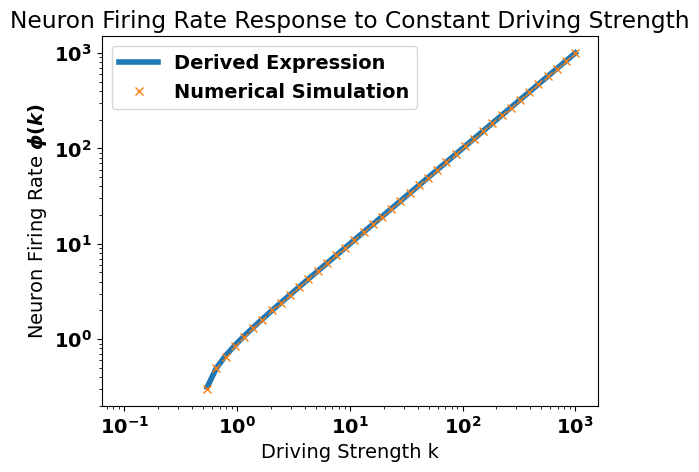
\includegraphics[width=\linewidth]{figures/phi_vs_k_const_driving.png}
\caption{A log-log plot of equation (\ref{eq:freq_vs_driving_strength_const}) alongside the rates measured from numerical simulations. The simulation parameters are described at the beginning of this section.  The rate was measured as the number of spike resets divided by the duration of the simulation. }\label{fig:spike_rate_vs_k_const_driving}
\end{figure}

The network will encode the constant driving force by spiking at a fixed rate determined by equation $(\ref{eq:freq_vs_driving_strength_const})$. Figure (\ref{fig:spike_rate_vs_k_const_driving}) shows a plot of equation (\ref{eq:freq_vs_driving_strength_const}) along with numerically computed spike rates for a simulated network driven with constant drive strength ratio $\frac{||k||}{||s||}$.  Similar to membrane voltage, the resulting slow feedback  and readout dynamics are reduced to one neuron periodically spiking:
\begin{align*}
\dot{\rho_1} &= -\rho_1 + \tilde{o}_1 \\ 
\\
\implies 
\dot{\hat{x}} &= - S_1 \rho_1 + S_1 \tilde{o}_1\\
\\ 
&= - \hat{x} + S_1 \tilde{o}_1,
\end{align*}
where $S_1 \in \mathbf{R}^{d}.$


\item The spike train $\tilde{o}_1$ is a periodic sequence of impulses spaced in time by $\frac{1}{\phi}$. If the first spike occurs at $\xi_1^1$, then $\tilde{o}_1(\xi) = \sum_{l=0}^{\infty} \delta \left(\xi-\xi_1^1 - \frac{l}{\phi}\right).$
The network estimate therefore has dynamics
\begin{align}
\label{eq:estimation_dynamics_const_driving}
\dot{\hat{x}} &= -\hat{x}  + S_1 \sum_{l=0}^{\infty} \delta \left(\xi - \frac{l}{\phi}\right).
\end{align}

The target dynamical system is
\begin{align*}
\dot{x} = - x + k 
\\
 x(0) = \begin{bmatrix} \frac{1}{2} & 0 \end{bmatrix},
\end{align*}
which has a stable fixed point at
\begin{align}
\label{eq:steady_state_dynamics_const_driving}
x = k.
\end{align}

Equation (\ref{eq:estimation_dynamics_const_driving}) implies that the network estimate $\hat{x}$ will decay until the first spike $\xi_1^1$ occurs:
\begin{align*}
\hat{x}(\xi) = x(0) e^{-\xi}, \hspace{4mm} 0 \leq \xi < \frac{1}{\phi}.
\end{align*}


 At this instant, the vector $S_1$ is added to the network estimate.
 \begin{align*}
 \hat{x}( \frac{1}{\phi}) =  x(0) e^{- \frac{1}{\phi}} + S_1.
 \end{align*}
 
Decay again occurs until the next spike
\begin{align*}
\hat{x}(\xi) &= \hat{x}(\frac{1}{\phi}) e^{-(\xi - \frac{1}{\phi})}, \\
\\
&= \left( x(0) e^{- \frac{1}{\phi}} + S_1 \right)e^{-(\xi - \frac{1}{\phi})} , \hspace{4mm} 
\frac{1}{\phi} \leq \xi < \frac{2}{\phi}\\
\\
\implies
\hat{x}(\frac{2}{\phi}) &= \left( x(0) e^{- \frac{1}{\phi}} + S_1 \right) e^{-(\frac{1}{\phi})} + S_1\\
\\
&= x(0)
e^{-\frac{2}{\phi}} + S_1 e^{-\frac{1}{\phi}} 
+ S_1.
\end{align*}

The third spike more clearly shows the recursive behavior
\begin{align*}
\hat{x}(\frac{3}{\phi}) &= \left[x(0)
e^{-\frac{2}{\phi}} + S_1 e^{-\frac{1}{\phi}} 
+ S_1\right] e^{-\frac{1}{\phi}} + S_1\\
\\
&= x(0) e^{-\frac{3}{\phi}} + S_1 e^{-\frac{2}{\phi}} 
+ S_1 e^{-\frac{1}{\phi}} + S_1
\end{align*}
Let us consider the $n^{th}$ spike sufficiently far from $\xi=0$ such that the transient term $x(0)e^{-\frac{n}{\phi}}$ can be neglected. This leads to the expression

\begin{align*}
\hat{x}(\frac{n}{\phi}) &= \sum_{l=0}^{n-1} S_1 e^{- \frac{l}{\phi}}  \\
\\
&= S_1 \frac
{ 1 - e^{-\frac{n}{\phi}}  }
{ 1 - e^{-\frac{1}{\phi}}  }.
\end{align*}

For sufficiently large $n$, this converges to 
\begin{align}
\label{eq:steady_state_estimate_const_driving}
\hat{x}(\xi_1^n) = \frac{S_1}{1 - e^{-\frac{1}{\phi}}}.
\end{align}


\begin{figure}[h]
\centering
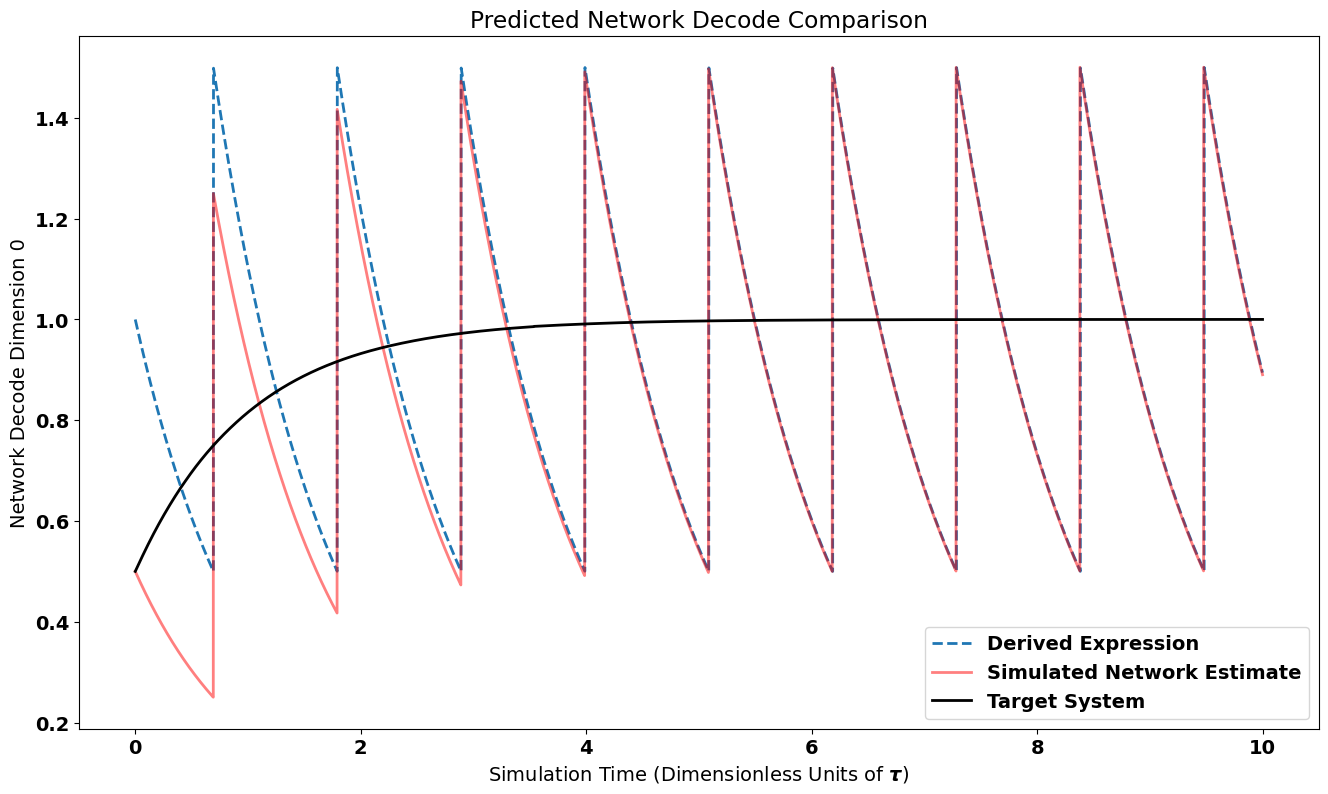
\includegraphics[width=\linewidth]{figures/network_decode_long_term_estimate.png}
\caption{Comparison of the derived long-term network estimate equation (\ref{eq:const_driving_network_estimate_explicit_expression_long_term}) to numerical simulation. Parameters are the same as the previous figure, with $\frac{||S_1||}{||k||} = 1$.}
\label{fig:const_driving_convergence_to_derived_spike_readout}
\end{figure}

\item The preceding argument states that after a transient interval, the network estimate at any spike time $\xi_1^n$ is given by equation (\ref{eq:steady_state_estimate_const_driving}). As shown in figure (\ref{fig:const_driving_convergence_to_derived_spike_readout}), this convergence occurs after roughly 5 spikes under the given parameters. 


We know from equation (\ref{eq:estimation_dynamics_const_driving}) that the estimate will decay exponentially from this value over an interval $\frac{1}{\phi}$ until a spike returns it returns to the initial value. Thus the network estimate between two consecutive spikes is given by 
\begin{align*}
\hat{x}(\xi) = \frac{S_1}{1 - e^{-\frac{1}{\phi}}} e^{-(\xi - \xi_1^n)}, \hspace{4mm} 0 \leq \xi - \xi_1^n  < \frac{1}{\phi}.
\end{align*}

Combine this expression with equation (\ref{eq:steady_state_estimate_const_driving}), we have an explicit expression for the long-term behavior of the network estimate given by 

\begin{equation}
\label{eq:const_driving_network_estimate_explicit_expression_long_term_phi}
\hat{x}(\xi) =
\frac{S_1}{1 - e^{-\frac{1}{\phi}}} e^{- (\xi - \xi_1^1) \mod{\frac{1}{\phi}}},
\end{equation} 
where $x \mod{y}$ denotes the fractional remainder of $x$ after division by $y$. 

Writing this equation in terms of provided network parameters, we use (\ref{eq:freq_vs_driving_strength_const}), to first obtain:
$$
e^{-\frac{1}{\phi}} = \left(\frac{2 k-\Lambda_1 S_1}{2 k+\Lambda_1 S_1}\right)^{1/\Lambda_1},
$$
which then gives
\begin{align}
\label{eq:const_driving_network_estimate_explicit_expression_long_term}
\hat{x}(\xi) =
\frac{S_1}
{
	\left(\frac{2 k-\Lambda_1 S_1}{2 k+\Lambda_1 S_1}\right)^{1/\Lambda_1}
}
 e^{- (\xi - \xi_1^1) \mod{\left(\frac{2 k+\Lambda_1 S_1}{2 k-\Lambda_1 S_1}\right)^{1/\Lambda_1}}}.
\end{align}


\item Assume the true system dynamics have settled to their fixed point $x = k$. From equation (\ref{eq:const_driving_network_estimate_explicit_expression_long_term}) the network estimate $\hat{x}$ and therefore error $e = x - \hat{x}$ is a periodic function of $\xi$ with period $\frac{1}{\phi}$. The RMSE over any integer number of spike periods is easily calculated from the RMSE over a single spike period. 

We compute the per-spike RMSE of the error signal  $e$ by 
\begin{equation}
\label{eq:per_spike_rmse_def}
RMSE_{spike} \overset{\Delta}{=} \sqrt{\phi \int_{0}^{\frac{1}{\phi}} \!  ||e(\tau)||^2 \, \, \mathrm{d}\tau}.
\end{equation}

The integrand $||e(\tau)||^2$ simplifies to 

\begin{align*}
e^T e &= (x - \hat{x})^T (x - \hat{x}) \\
\\
&= x^T x - 2 x^T \hat{x} + \hat{x}^T \hat{x} \\
\\
&= ||k||^2 \, - 2 S_1^T k \frac{e^{- \tau}}{1 - e^{-\frac{1}{\phi}}} 
+ 
||S_1||^2  \left(\frac{e^{- \tau}}{1 - e^{-\frac{1}{\phi}}} \right)^2\\
\\
&= ||k||^2 \, - 2 ||S_1|| \,  ||k|| \frac{e^{- \tau}}{1 - e^{-\frac{1}{\phi}}} 
+ 
||S_1||^2  \left(\frac{e^{- \tau}}{1 - e^{-\frac{1}{\phi}}} \right)^2.
\end{align*}

Note that
$$
\int_{0}^{\frac{1}{\phi}} \! e^{-\tau} \, \, \mathrm{d}\tau 
=
1-e^{-\frac{1}{\phi}},
$$

while 
\begin{align*}
\int_{0}^{\frac{1}{\phi}} \! \left(e^{-\tau}\right)^2
&=
\frac
{
	1 - e^{-\frac{2}{\phi}}
}
{2}
\\
\\
&= 
\frac{1}{2}\left(1 - e^{-\frac{1}{\phi}}\right)\left(1 + e^{-\frac{1}{\phi}}\right).
\end{align*}

Therefore the integral is

\begin{align*}
\phi\int_{0}^{\frac{1}{\phi}} \!  ||e(\tau)||^2 \, \, \mathrm{d}\tau &= 
||k||^2 -
   2\, \phi  \, ||S_1|| \, ||k|| 
   +
   \phi \,
   \frac{||S_1||^2}{2} 
	\frac{1+e^{-\frac{1}{\phi} }}{1-e^{-\frac{1}{\phi} }}
\end{align*}


The per-spike RMSE of the network estimate is thus
\begin{equation}
RMSE_{spike}(k, S_1, \phi) =
\sqrt
{
	||k||^2 -
	   2\, \phi  \, ||S_1|| \, ||k|| 
	   +
	   \phi \,   \frac{||S_1||^2}{2} 
	\frac{1+e^{-\frac{1}{\phi} }}{1-e^{-\frac{1}{\phi} }}
}.
\end{equation}

To write the RMSE explicitly as a function of given parameters $S_1, k, \Lambda_1$, we substitute our earlier expression for $e^{-\frac{1}{\phi}}$ and use equation (\ref{eq:freq_vs_driving_strength_const})to obtain
\begin{align}
\label{eq:per_spike_rmse_const_driving_ksl}
RMSE_{spike}(k, S_1, \Lambda_1) &=
\sqrt
{	
	||k||^2 -
	 2
	 \frac{ \, \Lambda_1 ||S_1|| \, ||k||}
	 {
	 	ln\left(\frac{2\,||k|| + \Lambda_1 ||S_1||}{2\,||k|| - \Lambda_1 ||S_1||}  \right)
	  }
	  + 
	  \frac{ \, \Lambda_1 }
	 {
	 	ln\left(\frac{2\,||k|| + \Lambda_1 ||S_1||}{2\,||k|| - \Lambda_1 ||S_1||}  \right)
	  }
	  \frac{||S_1||^2}{2}
	  \left(
	  \frac
	  {1 + \left(\frac{2 ||k||-\Lambda_1 ||S_1||}{2 ||k||+\Lambda_1 ||S_1||}\right)^{1/\Lambda_1} }
  	  {1 - \left(\frac{2 ||k||-\Lambda_1 ||S_1||}{2 ||k||+\Lambda_1 ||S_1||}\right)^{1/\Lambda_1} }
	  \right)
}
\end{align}

\item For the case where $\Lambda_1=-1$ and $S_1=1$, we can solve for the per-spike RMSE as a simple function of $\phi$.  First note that from equation (\ref{eq:freq_vs_driving_strength_const}),
$$
\frac{||k||}{||S_1||}\left(\phi\right) = 
\frac{1}{2} \,
\frac
{1+e^{-\frac{1}{\phi} }}
{1 - e^{-\frac{1}{\phi} }}.
$$

From the preceding expression equation (\ref{eq:per_spike_rmse_const_driving_ksl}) simplifies to 
%\label{eq:constant_driving:per_spike_rmse_vs_phi}
$$
RMSE_{spike}\left(k,S_1,\phi\right) =
\sqrt
{
	||k||^2 -
	    \phi ||S_1|| \, ||k||
}.
$$	   

If we normalize by the driving force $||k||$, we can isolate the change in network accuracy due to the intrinsic neuron firing rate. Divide the preceding expression by $||k||$ to get

\begin{equation}
\label{eq:constant_driving:per_spike_rmse_vs_phi}
NRMSE_{spike}\left(\phi\right) =
\sqrt
{
	1 -
	    2 \phi \frac
{1 - e^{-\frac{1}{\phi} }}
{1 + e^{-\frac{1}{\phi} }} 
}.
\end{equation}



Equations (\ref{eq:per_spike_rmse_const_driving_ksl}) and (\ref{eq:constant_driving:per_spike_rmse_vs_phi}) are plotted in figure (\ref{fig:const_driving_per_spike_rmse_vs_phi}). Note that the drive strength varies the amplitude of the target system's steady state. Thus we have derived the the network performance over its dynamic range of representable state space. 



\begin{figure}[h]
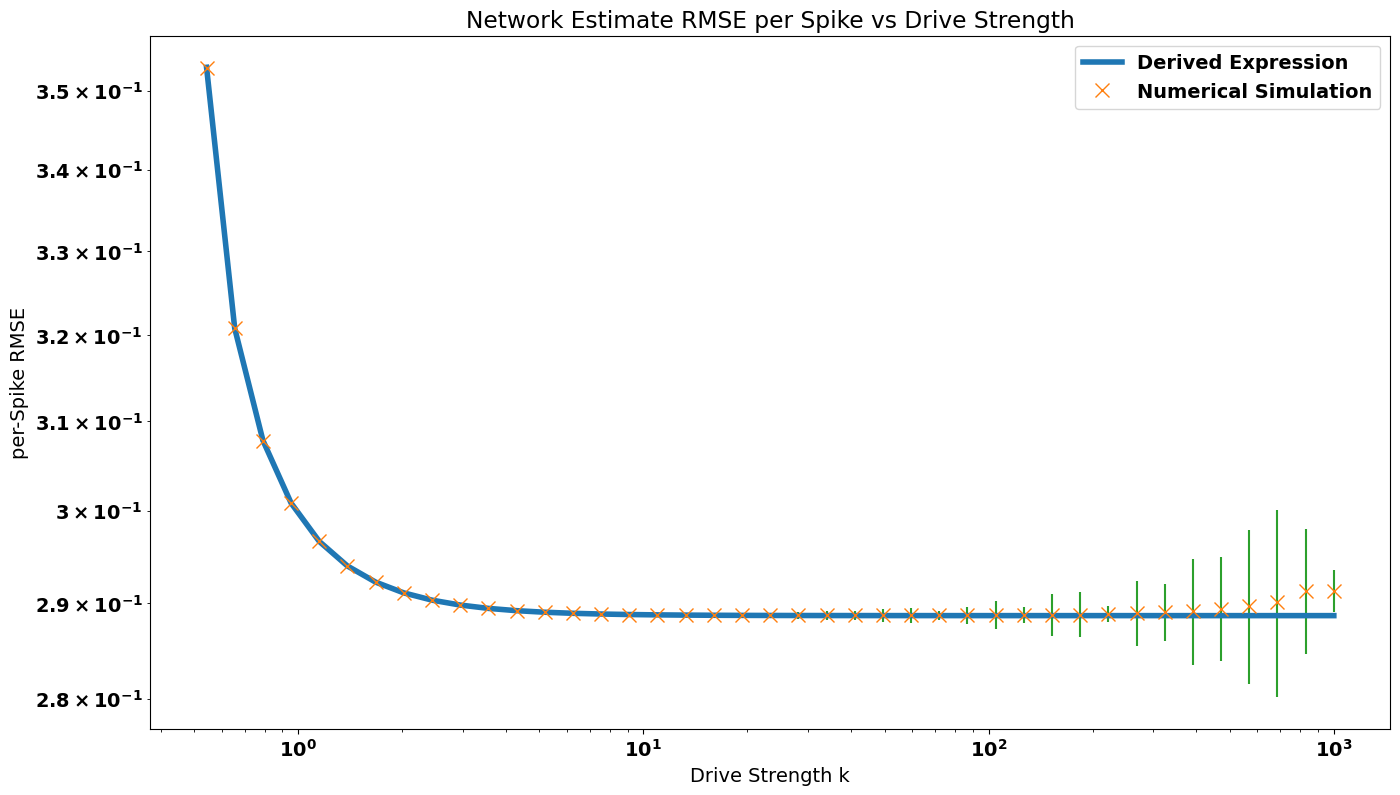
\includegraphics[width=\linewidth]{figures/rmse_sp_vs_k_const_driving.png}
\centering
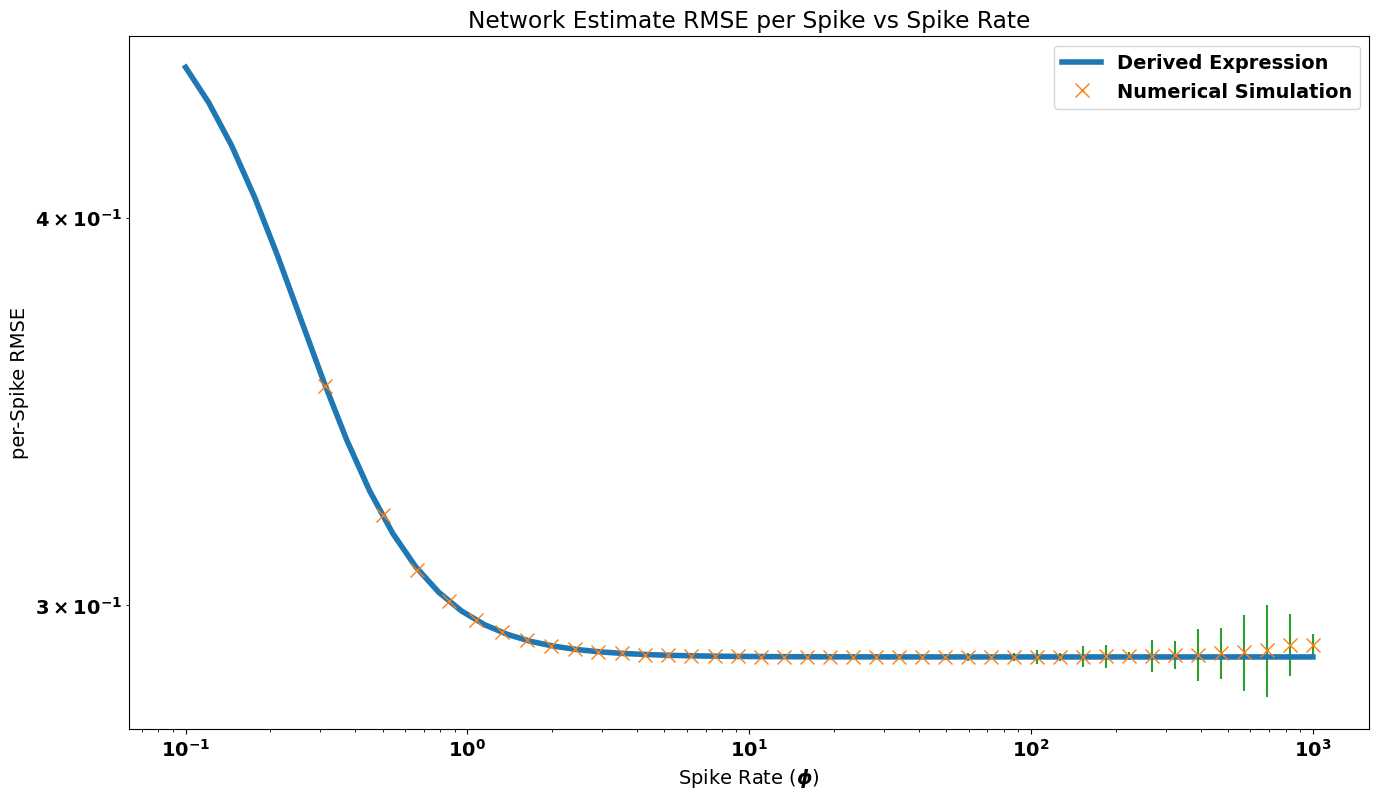
\includegraphics[width=\linewidth]{figures/rmse_sp_vs_phi_const_driving.png}
\caption{\textbf{\textit{Top:}} A log-log plot of equation (\ref{eq:per_spike_rmse_const_driving_ksl}). \textbf{\textit{Bottom:}} A log-log plot of equation (\ref{eq:constant_driving:per_spike_rmse_vs_phi}). \textbf{\textit{Both:}} Each simulated data point is the RMSE averaged over all inter-spike intervals in a simulation of length $T = 80 \tau_s$ at a constant (in time) drive strength. Between simulations, the spike rates were varied by sweeping drive strength. Green vertical lines towards the larger values are +/- 1 standard deviation. The spike rates $\hat{\phi}$ were computed numerically via dividing the number of spikes in a simulation by the simulation duration. The RMSE between two adjacent spikes was computed by numerical integration as a discrete sum: $\hat{RMSE} = \sqrt{\hat{\phi} \sum_{\tau \text{ between spikes }} e(\xi)^T e(\xi) \, \, d\xi }$.}
\label{fig:const_driving_per_spike_rmse_vs_phi}
\end{figure}
\end{enumerate}
